% ====================================================================
%
% LSST DESC DC2 Data Release Note
%
% ====================================================================

\documentclass[11pt]{report}


\usepackage{datetime}
\usepackage{fancyhdr}
\usepackage[outermarks]{titlesec}
\usepackage[utf8x]{inputenc}
\usepackage[T1]{fontenc}
\usepackage{amsmath}
\usepackage{amssymb}
\usepackage{epsfig}
\usepackage{graphics}
\usepackage{graphicx}
\usepackage[usenames]{color}
\usepackage{helvet}
\usepackage{times}
\usepackage{natbib}
\usepackage{import}
\usepackage{tabularx}
\usepackage{xspace}
\usepackage{scrextend}
%\usepackage{parskip}
\usepackage[normalem]{ulem}
\usepackage{scrwfile} % Stops "No room for a new \write" complaint
\usepackage{xcolor}
\usepackage{colortbl}
% Big tables summarizing plans:
\usepackage{pdflscape}
\usepackage{afterpage}

\usepackage{pdftexcmds}

% Hyperref - always load as the last package!
\usepackage[linktocpage=false]{hyperref}
\hypersetup{
    colorlinks=true,
    citecolor=DESCred,
    filecolor=DESCred,
    linkcolor=DESCred,
    urlcolor=DESCred,
}
\usepackage{hypcap}
\usepackage{inconsolata}
%%%%%%%%%%%%%%%%%%%%%%%%%%%%%%%%%%%%%%%%%%%%%%%
% Cross-references

\renewcommand*{\figureautorefname}{Figure}
\renewcommand*{\tableautorefname}{Table}
\renewcommand*{\equationautorefname}{Equation}
\renewcommand*{\sectionautorefname}{Section}
\renewcommand*{\subsectionautorefname}{Section}
\renewcommand*{\subsubsectionautorefname}{Key~Project}
\renewcommand*{\paragraphautorefname}{Deliverable}
\renewcommand*{\subparagraphautorefname}{Key~Task}
\renewcommand*{\appendixautorefname}{Appendix}

%%%%%%%%%%%%%%%%%%%%%%%%%%%%%%%%%%%%%%%%%%%%%%%
\def\bfseries{\fontseries \bfdefault \selectfont \boldmath} % make math mode bold in section titles
\renewcommand{\thesection}{\arabic{section}}
\setcounter{secnumdepth}{5}
%%%%%%%%%%%%%%%%%%%%%%%%%%%%%%%%%%%%%%%%%%%%%%%
%  make \paragraph and \subparagraph behave like other section commands
% THIS IS FROM THE DESI SRP.

    \titleformat{\section}
      {\normalfont\large\bfseries}{\thesection}{1em}{}
    \titleformat{\subsection}
      {\normalfont\normalsize\bfseries}{\thesubsection}{1em}{}
    \titleformat{\subsubsection}
      {\normalfont\normalsize\bfseries}{\thesubsubsection}{1em}{}
    \titleformat{\paragraph}
      {\normalfont\normalsize\bfseries}{\theparagraph}{1em}{}
    \titleformat{\subparagraph}
      {\normalfont\normalsize\bfseries}{\thesubparagraph}{1em}{}

    \titlespacing\section{0pt}{12pt plus 4pt minus 2pt}{0pt plus 2pt minus 2pt}
\titlespacing\subsection{0pt}{12pt plus 4pt minus 2pt}{0pt plus 2pt minus 2pt}
\titlespacing\subsubsection{0pt}{12pt plus 4pt minus 2pt}{0pt plus 2pt minus 2pt}

%%%%%%%%%%%%%%%%%%%%%%%%%%%%%%%%%%%%%%%%%%%%%%%

\linespread{1.1}
 \addtolength{\hoffset}{-0.0cm}
 \setlength{\topmargin}{-0.in}
 \setlength{\textheight}{8.25in}
\setlength{\footskip}{1.5cm} %{0.75cm}
\setlength{\textwidth}{6.25in}
\setlength{\evensidemargin}{1in}
\setlength{\oddsidemargin}{0in}

%  \usepackage{paralist}
%\setlength{\pltopsep}{0pt}
%\setlength{\plpartopsep}{0pt}

\def\tcr{\textcolor{red}}
\def\tcb{\textcolor{blue}}
\def\accent{\it}
\def\vs{\vspace{0.5cm}}
\def\hs{\hspace{0.5cm}}
\urlstyle{rm}
 % formatting for doc, copied from SRM

%%%%% MACROS AND SETTINGS FOR CS REPORTS

%=====================================================================
% SET UP RECOMMENDATION COMMANDS
%
% Adapted from Science Roadmap file, Rachel Bean & Phil Marshall Summer 2015
% Based on commands written by Daniel Einsenstein for DESI SRP April 2015
%=====================================================================
\usepackage{xifthen}
\usepackage{xspace}

% Number tables and figures by section
\let\counterwithout\relax
\let\counterwithin\relax
\usepackage{chngcntr}
\counterwithin{table}{section}
\counterwithin{figure}{section}

\usepackage{multirow}
% Enable sensible resizing of lists of projects and recommendations:
\usepackage{tocloft}
\renewcommand\cftparafont{\small}
\renewcommand\cftparapagefont{\small}
\renewcommand\cftsubparafont{\footnotesize}
\renewcommand\cftsubparapagefont{\footnotesize}

% for \autoref
\renewcommand*\sectionautorefname{Section}
\renewcommand*\subsectionautorefname{Section}
\renewcommand*\subsubsectionautorefname{Section}


\usepackage{datetime}

%\newcommand{\docheader}{{LSST DESC Operations Plan}}

% --------------------------------------------------------------------

\makeatletter

% --------------------------------------------------------------------
% REFERENCING COMMANDS

% Include down to the subsection level in the table of contents:
\setcounter{tocdepth}{2}

% \counterwithin{section}{chapter}
% \counterwithin{table}{chapter}
% \counterwithin{figure}{chapter}

\renewcommand*{\chapterautorefname}{Chapter}
\renewcommand*{\appendixautorefname}{Appendix}
\newcommand{\appref}[1]{\hyperref[#1]{Appendix~\ref{#1}}}

\newcommand{\relabel}[3]{\@bsphack
    \protected@write\@auxout{}%
        % {\string\newlabel{#2}{{#1}{#3}{\relax}{#2}{}}}%
        {\string\newlabel{#2}{{#1}{\thepage}{\relax}{#3}{}}}%
    \@esphack}

% --------------------------------------------------------------------

% POINT OF CONTACT

% Contact list - repo in URL must be set correctly to enable queries to be made:
\newcommand{\contact}[2]{%
\href{https://github.com/LSSTDESC/CosmologicalSimulationsPlan/issues/new?title=Question:\%20\&body=#2:\%20}{{\it #1}}%
}
\newcommand{\dontcontact}[2]{{\it #1}}

% Link to issue thread:
\newcommand{\issue}[1]{%
\href{https://github.com/LSSTDESC/CosmologicalSimulationsPlan/issues/#1}{\#{#1}}%
}


% --------------------------------------------------------------------

% USEFUL MACROS

% The \todo macro can be used to mark missing items or to pose questions to the group.
\newcommand{\todo}[1]{\noindent{\textcolor{red}{[TODO: #1]}}}
\newcommand{\toask}[1]{\noindent{\textcolor{magenta}{[Q for #1]}}}
\newcommand{\note}[1]{\noindent{\textcolor{blue}{[#1]}}}


% Uncomment the following line to make the \todo items invisible.
%\renewcommand\todo[1]{\relax}

% List of Recommendations, using Table of Contents commands:
\newcommand{\listofrecommendations}{
  \@starttoc{tor}
}

% For inline code (like `...` in markdown)
\DeclareUrlCommand\code{\urlstyle{tt}}

% List of projects, designed to act as a table of contents in each
% section:
\newcommand{\listofjusttheserecommendations}[1]{
  \vskip\baselineskip
  {\bf \nameref{sec:\headerstring} Recommendations:}
  \phantomsection\label{tab:\headerstring:recommendations}
  \medskip
  \hrule
  % \@starttoc{#1}
  \@starttoc{\headerstring.tor}
  \hspace{-0.5em}
  \medskip
  \hrule
  \vskip\baselineskip
  \vskip\baselineskip
}

% --------------------------------------------------------------------

% COUNTERS AND VARIABLES:

\newcounter{recommendation}

\newcommand{\resetnumbering}{
   \setcounter{subsubsection}{0}
   \setcounter{paragraph}{0}
   \setcounter{subparagraph}{0}
   \setcounter{equation}{0}
   \setcounter{recommendation}{0}
}

% Prefix section title
\newcommand{\sectionstring}{}
% Prefix for key projects and recommendations in each section (SL, WL etc)
\newcommand{\headerstring}{}
% Recommendations are organised by sections, whose names
% are used in formatting the titles etc. ENV, FRW, WKF, OPS

\def\myaddcontentsline#1#2#3#4{\addtocontents{#1}{\protect\contentsline{#2}{#3}{#4}{}}}

% --------------------------------------------------------------------

% TABLE OF CONTENTS

\newcommand{\maketoc}{
   \renewcommand{\contentsname}{\hrule{\large\flushleft\sffamily\bfseries Contents\vspace{-1.2cm}}}
   \setlength{\parskip}{0.1cm}
   \phantomsection\tableofcontents % PJM: phantom section is needed to give \label something to point at.
   \flushbottom
   \vs\hrule
}


% --------------------------------------------------------------------

% RECOMMENDATION COMMANDS

%%% Recommendations should be phrased as verbs
%%% Recommendations have one argument: a title

%%% Use \recommendation[tag]{title}
%%% \recommendationref{tag} will echo the recommendation number
%%% \pageref{tag} will return the recommendation number

% \recommendationnum is used for labeling recommendations. Since recommendations
% belong to charge area, their numbers include the headerstring (eg "FW")
% "\recommendationnum" -> "FW:1"
\newcommand{\recommendationnum}{%
    \headerstring:\therecommendation
}

% \recommendationstring is how the recommendation title will appear in the text.
% "\recommendation[no-windows]{Don't Support Windows}"
%     -> "Recommendation ENV:1 - Don't Support Windows"
% The hyperlink takes you to the list of recommendations, so you can see it in context
\newcommand{\recommendationstring}[2]{\hyperref[tor:\recommendationnum]{\textbf{Recommendation \recommendationnum: We should #2}}}
% Version without hyperlink to list of recommendations:
% \newcommand{\recommendationstring}[2]{\textcolor{DESCred}{\textbf{Recommendation \recommendationnum -- #2}}}

% \recommendationliststring is how the recommendation title will appear in
% the list of recommendations.
%     -> "ENV:1 – Don't Support Windows"
% The hyperlink takes you to the start of the recommendation text.
\newcommand{\recommendationliststring}[1]{\hyperref[\thisrecommendationname]{\textbf{\recommendationnum}} -- we should #1}

% \recommendationrefstring is the text that will appear when a recommendation is cited.
% "recommendation~\recommendationref{no-windows}"  -> "recommendation ENV:1"
\newcommand{\recommendationrefstring}{\recommendationnum}

% \printrecommendation is used to write the recommendation title line itself.
\newcommand{\printrecommendation}[1]{\noindent{#1}}

% \recommendationref is the function to use when referring to a recommendation.
\newcommand{\recommendationref}[1]{\noindent \ref{#1}}

% Which section's table are we goingto be adding to?
\newcommand{\recommendationtable}{\headerstring.tor}

% \makerecommendation is run when \recommendation{} is called. Note the
% use of the paragraph counter to provide an anchor for hyperref.

\newcommand{\makerecommendation}[3]{
   \stepcounter{recommendation}
   \vskip 0.2in
   \refstepcounter{paragraph} % This puts an anchor right before the title line.
   % Write the recommendation title and summary:
   \printrecommendation{\recommendationstring{#1}{#2}}
   \newline\noindent{{\it {#3}}}
   \vskip 0.2in
   % Add line to list of all recommendations, including a label to point to:
   % \addcontentsline{tor}{recommendation}{\small\printrecommendation{\recommendationliststring{#2}}\hfill}
   \addcontentsline{tor}{recommendation}{\leavevmode\newline\small\printrecommendation{\recommendationliststring{#2}}\hfill\protect\phantomsection\protect\label{tor:\recommendationnum}}
   % \myaddcontentsline{tor}{recommendation}{\small\printrecommendation{~~~~\recommendationliststring{#2}}\hfill}{#1}
   % Add line to this sections's table of recommenandations:
   \addcontentsline{\recommendationtable}{recommendation}{\leavevmode\newline\small\printrecommendation{\recommendationliststring{#2}}\hfill}
}

% The recommendation command itself - make a new recommendation (which prints
% a title line, advances the paragraph counter, then prints the summary) and label it for
% referring to it elsewhere.
\newcommand{\recommendation}[3][]{
   \def\thisrecommendationname{#1}
   \def\thisrecommendationtitle{#2}
   \def\thisrecommendationsummary{#2}
   \makerecommendation{#1}{#2}{#3}
   \relabel{\recommendationrefstring}{#1}{paragraph.\thechapter.\theparagraph}
 }


% --------------------------------------------------------------------

% NAVIGATION

\newcommand{\footernavigationbar}
{
    \it\footnotesize Go to:
    \hyperref[toc]{The Table Of Contents} % Table of Contents
    \ifthenelse{\equal{\headerstring}{}}
   	    {}
        {
        	% $\bullet$ \nameref{sec:\headerstring}
            $\bullet$ \hyperref[sec:\headerstring]{the start of this section}
  			$\bullet$ \hyperref[sec:TOR]{the list~of~recommendations}
        }
}

\newcommand{\quickref}[1]{\ref{#1}~\nameref{#1}}

% --------------------------------------------------------------------



%%%%%%%%%%%%%%%%%%%%%%%%%%%%%%%%%%%%%%%%%%%%%%%%%%%%%%%%%%%%%%%%%%%%%%

% Other useful dates:

% US financial years. The first quarter, Q1,
% is taken to be Sept, Oct and Nov. The end of 2017 Q1 would be 11/17.
% Starts of Q1,Q2,Q3,Q4 -> 09/Y-, 12/Y-, 03/YY, 06/YY
%   Ends of Q1,Q2,Q3,Q4 -> 11/Y-, 02/Y-, 05/YY, 08/YY
% This macro works correctly in the text, but cannot be used in place of a
% datestring argument (#1) in the \recommendation command. I (PJM) don't
% know why.
\newcommand{\FY}[2]{%
% eg \FY{16}{1} -> "11/15"
\newcount\year
\ifthenelse{\equal{#2}{Q1}}%
{%
  \year=\numexpr#1-1\relax
  {11/\the\year}%
}{%
  \year=#1%
  \ifthenelse{\equal{#2}{Q2}}{02/\the\year}{%
  \ifthenelse{\equal{#2}{Q3}}{05/\the\year}{%
  {08/\the\year}%
}}}%
}



\newcommand{\deadline}[1]{%
% Parse the datestring provided. Possible options are '??/??',
% '05/17', '5/17', DC1, etc. Default is that date string is
% passed through as is. '??/??' needs
% processing, though.
%
% Relative dates, passed in by keywords like "DC1", will appear in
% regular (not bold) type, to show that they might change with the
% collaboration's schedule.
%
% "DC1" is interpreted to mean the end of the data analysis of DC1.
% Later on we might think about allowing more complex arguments, such as
% "DC1-analysis-start".
%
% US financial years are assumed, so that the first quarter, Q1,
% is taken to be Sept, Oct and Nov. The end of 2017 Q1 would be 11/17.
% Q1,Q2,Q3,Q4 -> 11, 2, 5, 8
%
% First set the correct era.
% This is the big one: any undefined date gets set to the end of
% the current key project's data challenge era:
\ifthenelse{\equal{#1}{??/??}}%
    {\def\era{\thisrecommendationsera}}%
    {\def\era{#1}}%
% This works correctly: era is now either set to "DC1", "DC2" or "DC3"
% (if "??/??" was chosen), or the argument provided.
%
% Inputs to the \recommendation date argument can themselves be macros,
% for example:
%   \recommendation[D:SL-DC1-TDC2:DP1]{\EndofDCOneDC}{\SLTDCtwo Simulated Light Curves}
% This is the preferred way of passing in this information.
% You can also pass in one of the DC names, and it will be
% interpreted as the end date of that DC era, as set by DESC mgmt above.
% This will get set in lightweight font, because its a pretty
% vague timeline!
\ifthenelse{\equal{\era}{DC1}}{\def\duedate{\EndofDCOne}}{%
\ifthenelse{\equal{\era}{DC2}}{\def\duedate{\EndofDCTwo}}{%
\ifthenelse{\equal{\era}{DC3}}{\def\duedate{\EndofDCThree}}{%
% Now we get to the situation where the date was either
% explicitly set, or left as ??/??. The question marks should
% be replaced with \thisrecommendationsera, but if this has happened,
% we set the date in lightweight font. An explicit due date setting is
% set in bold.
\ifthenelse{\equal{#1}{??/??}}{\def\duedate{\era}}{%
% else: the date was set by hand.
\def\duedate{{\bf{\era}}}%
% The following line closes this huge nested if block. There must
% be as many '}' characters on this line as there are 'ifthenelse'
% lines above.
}}}}
% Finally, render the due date, as a hyperlink to the timeline chart:
\hyperref[fig-DC]{\duedate}
}% End of \deadline macro.


% Possible extensions to \deadline
% --------------------------------
%
% Automatically detect the recommendation type from a name like
% "D:KPNAME:TYPE:NUMBER" - which would need all recommendation names to
% follow this convention, probably...
% Splitting strings:
%   http://tex.stackexchange.com/questions/12810/how-do-i-split-a-string
%
% Parse deadlines like DC1-analysis-end?
%
%   Need to be able to split a string like "05/17" and subtract 7 months
%   from it.
%
% Enabling dates minus some number of months?
%
%   See the following for arithmetic in latex:
%   http://tex.stackexchange.com/questions/133317/how-to-add-subtract-multiply-and-divide-in-plain-tex
%
% --------------------------------------------------------------------

% Bibliography stuff:

\bibpunct[, ]{(}{)}{;}{a}{}{,}

% Rename bibliography sections and make everything more compact:
\renewcommand\bibname{\normalsize References}

% PJM (for the Science Book): This command makes latex set up the bibliography as a section*, not
% a chapter. Need to add a markboth command too, below...
% PJM (for the SRM): Not sure this is working...
% \renewcommand\bibsection{\chapter*{\refname}}
\renewcommand\bibsection{\section*{\refname}}
% PJM 10/10/09: need this switch to change marking of appendix headers:
\newboolean{appendix}
\setboolean{appendix}{false}

\let\oldthebibliography=\thebibliography
\let\endoldthebibliography=\endthebibliography
\renewenvironment{thebibliography}[1]{%
  \begin{oldthebibliography}{#1}%
    % Make sure the references line gets into the contents table - note spacing!
    % \addcontentsline{toc}{chapter}{\hspace{2em}References}
    \addcontentsline{toc}{section}{References}
    % \footnotesize
    % \setlength{\parskip}{0ex}%
    % \setlength{\itemsep}{0ex}%
    % PJM 10/10/09: Appendix reference section headers need to be marked with
    % "Appendix" not "Chapter"
    % \ifthenelse{\boolean{appendix}}{
    %   \markboth{Appendix\ \thechapter: References}{Appendix\ \thechapter: References}
    % }{
    %   \markboth{Chapter\ \thechapter: References}{Chapter\ \thechapter: References}
    % }
}%
{%
  \end{oldthebibliography}%
}

%=====================================================================

\makeatother

%=====================================================================
% Add your macros here for all to use!

% LSST Project terminology:
\newcommand{\LevelTwo}{{Level~2}\xspace}
\newcommand{\LevelThree}{{Level~3}\xspace}
\newcommand{\CC}{LSSTComCam\xspace}
\newcommand{\MultiFit}{{\sc MultiFit}\xspace}
\newcommand{\photoz}{photo-$z$\xspace}
\newcommand{\Nbody}{$N$-body\xspace}


% DESC-related software
\newcommand{\astropy}{{\sc astropy}\xspace}
\newcommand{\CAMB}{{\sc CAMB}\xspace}


% Image simulation tools:
\newcommand{\PhoSim}{{\sc PhoSim}\xspace}
\newcommand{\OpSim}{{\sc OpSim}\xspace}
\newcommand{\CatSim}{{\sc CatSim}\xspace}
\newcommand{\GalSim}{{\sc GalSim}\xspace}

% Data Products used by more than one WG
\newcommand{\DADConeHalocat}{\hyperref[KP:DA-DC1-HC]{{\bf\texttt{HaloCat}}}\xspace}%{{\bf\texttt{HaloCat\,1.0}}}\xspace}
\newcommand{\DATwinklesone}{\hyperref[KP:DA-DC1-TW1]{{\bf\texttt{Twinkles\,1}}}\xspace}%{{\bf\texttt{Twinkles\,1.0}}}\xspace}
\newcommand{\DATwinklestwo}{\hyperref[KP:DA-DC2-TW2]{{\bf\texttt{Twinkles\,2}}}\xspace}%{{\bf\texttt{Twinkles\,2.0}}}\xspace}
\newcommand{\DADCtwomockLC}{\hyperref[KP:DA-DC2-LC]{{\bf\texttt{DC2 Mock Lightcone}}}\xspace}
\newcommand{\DADCthreemockCC}{\hyperref[KP:DA-DC3-CC]{{\bf\texttt{DC3 Mock ComCam Survey}}}\xspace}
\newcommand{\DADCthreemockLC}{\hyperref[KP:DA-DC3-LC]{{\bf\texttt{DC3 Mock Lightcone}}}\xspace}
\newcommand{\DADConeDeep}{\hyperref[KP:DA-DC1-PHO-D]{{\bf\texttt{DC1 Phosim Deep}}}\xspace}
\newcommand{\DADConeWide}{\hyperref[KP:DA-DC1-PHO-W]{{\bf\texttt{DC1 Phosim Wide}}}\xspace}
\newcommand{\DADCtwoWide}{\hyperref[KP:DA-DC2-PHO-W]{{\bf\texttt{DC2 Phosim Wide}}}\xspace}
%\newcommand{\DADCtwomocks}{\hyperref[KP:DA-DC2-mock]{{\bf\texttt{DESC DC2 Mock Galaxy Catalogs}}}\xspace}
%\newcommand{\DAGREAT}{\hyperref[KP:DA-DC1-GREAT]{{\bf\texttt{GREAT DESC}}}\xspace}
% Weak Lensing software tools:
\newcommand{\WLImSim}{\hyperref[tab:WL:software]{\sc WLImSim}\xspace}
\newcommand{\WLShearPipe}{\hyperref[tab:WL:software]{\sc WLShearPipe}\xspace}
\newcommand{\WLTwopoint}{\hyperref[tab:WL:software]{\sc WLTwopoint}\xspace}
\newcommand{\WLNullTest}{\hyperref[tab:WL:software]{\sc WLNullTest}\xspace}
\newcommand{\WLCosmo}{\hyperref[tab:WL:software]{\sc WLCosmo}\xspace}
\newcommand{\WLMagPipe}{\hyperref[tab:WL:software]{\sc WLMagPipe}\xspace}
\newcommand{\WLNPoint}{\hyperref[tab:WL:software]{\sc WLNPoint}\xspace}
\newcommand{\WLBlendBias}{\hyperref[tab:WL:software]{\sc WLBlendBias}\xspace}
% LSS definition
\newcommand{\LSScatalog}{\hyperref[tab:LSS:software]{\sc LSScatalog}\xspace}
\newcommand{\LSStwopoint}{\hyperref[tab:LSS:software]{\sc LSStwopoint}\xspace}
\newcommand{\LSSthreepoint}{\hyperref[tab:LSS:software]{\sc LSSthreepoint}\xspace}
\newcommand{\LSSsyspre}{\hyperref[tab:LSS:software]{\sc LSSsyspre}\xspace}
\newcommand{\LSSsyshunter}{\hyperref[tab:LSS:software]{\sc LSSsyshunter}\xspace}
\newcommand{\LSSCross}{\hyperref[tab:LSS:software]{\sc LSSCross}\xspace}
\newcommand{\LSSCosmo}{\hyperref[tab:LSS:software]{\sc LSSCosmo}\xspace}

% Galaxy Clusters software tools
\newcommand{\CLOptCat}{\hyperref[tab:CL:software]{\sc CLOptCat}\xspace}
\newcommand{\CLFinder}{\hyperref[tab:CL:software]{\sc CLFinder}\xspace}
\newcommand{\CLPanCat}{\hyperref[tab:CL:software]{\sc CLPanCat}\xspace}
\newcommand{\CLRedshift}{\hyperref[tab:CL:software]{\sc CLRedshift}\xspace}
\newcommand{\CLSmurfs}{\hyperref[tab:CL:software]{\sc CLSmurfs}\xspace}
\newcommand{\CLMassMod}{\hyperref[tab:CL:software]{\sc CLMassMod}\xspace}
\newcommand{\CLShear}{\hyperref[tab:CL:software]{\sc CLShear}\xspace}
\newcommand{\CLAbsMass}{\hyperref[tab:CL:software]{\sc CLAbsMass}\xspace}
\newcommand{\CLRelMass}{\hyperref[tab:CL:software]{\sc CLRelMass}\xspace}
\newcommand{\CLForecast}{\hyperref[tab:CL:software]{\sc CLForecast}\xspace}
\newcommand{\CLCosmo}{\hyperref[tab:CL:software]{\sc CLCosmo}\xspace}

% Supernova software tools
%   [we can't let SL be the only ones with cool-looking names]
\newcommand{\SNRealizer}{\hyperref[tab:SN:software]{\sc SupernovaRealizer}\xspace}
\newcommand{\SNMonitor}{\hyperref[tab:SN:software]{\sc SupernovaMonitor}\xspace}
\newcommand{\SNType}{\hyperref[tab:SN:software]{\sc SupernovaType}\xspace}
\newcommand{\SNDistance}{\hyperref[tab:SN:software]{\sc SupernovaDistance}\xspace}
\newcommand{\SNCadence}{\hyperref[tab:SN:software]{\sc SupernovaCadence}\xspace}

% Photo-z software tools
\newcommand{\PZGalaxyGenerator}{\hyperref[tab:PZ:software]{\sc PZGalaxyGenerator}\xspace}
\newcommand{\PZPDF}{\hyperref[tab:PZ:software]{\sc PZPDF}\xspace}
\newcommand{\PZCalibrate}{\hyperref[tab:PZ:software]{\sc PZCalibrate}\xspace}
\newcommand{\PZSpeczSelector}{\hyperref[tab:PZ:software]{\sc PZSpeczSelector}\xspace}
%Photo-z Datasets
\newcommand{\PZColor}{\hyperref[KP:PZ:DC12]{\bf\texttt{PZColor}}\xspace}
\newcommand{\PZIncomplete}{\hyperref[KP:PZ:DC12]{\bf\texttt{PZIncomplete}}\xspace}
\newcommand{\PZCrossCorr}{\hyperref[KP:PZ:DC2_cor]{\bf\texttt{PZCrossCorr}}\xspace}
\newcommand{\PZSzTrain}{\hyperref[KP:PZ:ext_spec]{\bf\texttt{PZSzTrain}}\xspace}
\newcommand{\PZNIR}{\hyperref[KP:TJP-DC3-kp3]{\bf\texttt{PZNIR}}\xspace}

% Strong Lensing software tools:
\newcommand{\SLFinder}{\hyperref[tab:SL:software]{\sc SLFinder}\xspace}
\newcommand{\SLMonitor}{\hyperref[tab:SL:software]{\sc SLMonitor}\xspace}
\newcommand{\SLTimer}{\hyperref[tab:SL:software]{\sc SLTimer}\xspace}
\newcommand{\SLMassMapper}{\hyperref[tab:SL:software]{\sc SLMassMapper}\xspace}
\newcommand{\SLEnvCounter}{\hyperref[tab:SL:software]{\sc SLEnvCounter}\xspace}
\newcommand{\SLModeler}{\hyperref[tab:SL:software]{\sc SLModeler}\xspace}
\newcommand{\SLCosmo}{\hyperref[tab:SL:software]{\sc SLCosmo}\xspace}
% Strong Lensing datasets:
\newcommand{\SLTDCtwo}{\hyperref[KP:SL-DC1-TDC2]{\texttt{TDC2}}\xspace}
\newcommand{\SLTDCthree}{\hyperref[KP:SL-DC3-TDC3]{\texttt{TDC3}}\xspace}
\newcommand{\SLDCtwoReal}{\hyperref[]{\texttt{DC2 Real Data}}\xspace}
% Theory / Joint Probes software tools
\newcommand{\TJPForecast}{\hyperref[tab:TJP:software]{\sc TJPForecast}\xspace} % Joint probe covariance matrix
\newcommand{\TJPCosmo}{\hyperref[tab:TJP:software]{\sc TJPCosmo}\xspace} % Joint probe covariance matrix
\newcommand{\TJPCov}{\hyperref[tab:TJP:software]{\sc TJPCov}\xspace} % Joint probe covariance matrix

% Cosmology analysis tools
\newcommand{\CosmoSIS}{{\sc CosmoSIS}\xspace}
\newcommand{\CosmoLike}{{\sc CosmoLike}\xspace}

% Journals
\newcommand{\apj}{ApJ}
\newcommand{\apjl}{ApJL}
\newcommand{\apjs}{ApJS}
\newcommand{\mnras}{MNRAS}
\newcommand{\apss}{Ap \& SS}
\newcommand{\aap}{A\&A}
\newcommand{\aaprlong}{Astronomy and Astrophysics Reviews}
\newcommand{\aj}{AJ}
\newcommand{\prd}{Phys. Rev. D}
\newcommand{\nat}{Nature}
\newcommand{\araa}{ARA\&A}
\newcommand{\jgr}{J. Geophys. Res.}
\newcommand{\pasp}{PASP}
\newcommand{\aapr}{AAPR}
\newcommand{\jcap}{JCAP}
\newcommand{\pasj}{PASJ}

% Bits and pieces
\newcommand{\etal}{et~al.~}
\newcommand{\eg}{{\it e.g.\ }}
\newcommand{\ie}{{\it i.e.\ }}
\newcommand{\etc}{{\it etc.\ }}
\newcommand{\dndmag}{d$N$/dmag}
\newcommand{\neff}{\ensuremath{n_\text{eff}}}

% Colors, commenting etc:
\definecolor{gray}{rgb}{0.5,0.5,0.5}
\definecolor{green}{rgb}{0.0,0.5,0.0}
\definecolor{DESCred}{rgb}{0.63,0.00,0.20} % {#A10034}
\definecolor{dkblue}{rgb}{0, 0.30, 0.99 }%{0,76,253}
% Guidance at http://latexcolor.com/
% \newcommand{\question}[2]{\textcolor{red}{\bf Question from #1: #2}}
\newcommand{\flag}[2]{\textcolor{red}{\bf #1: #2}}
% \newcommand{\new}[1]{\textcolor{green}{#1}}
\newcommand{\black}[1]{\textcolor{black}{#1}}
\newcommand{\gray}[1]{\textcolor{gray}{#1}}

%\newcommand{\new}[1]{\textcolor{blue}{#1}}
%\newcommand{\question}[2]{\textcolor{blue}{{\bf Question from #1: #2}}} % eg \question{PJM}{Shouldn't this be ``better''?}
%\newcommand{\comment}[2]{\textcolor{blue}{{\bf #1: #2}}} % eg \comment{RXD}{This will likely be too expensive.}
\newcommand{\hlt}[1]{\textcolor{blue}{{#1}}}

% Cross-referencing definitions:
\newcommand{\define}[1]{\textcolor{DESCred}{\it{\bf #1}}\phantomsection\label{#1}}
\newcommand{\lookup}[1]{\hyperref[#1]{#1}}

%=====================================================================

\newcounter{requirementh}
\newcounter{requirementd}
\newcounter{objectives}
\newcounter{goal}
\newcommand{\probe}{\@empty}

\newcommand{\requirementhname}{%
    RH{\therequirementh}%
}
\newcommand{\requirementdname}{%
    \probe{\therequirementd}%
}
\newcommand{\objectivename}{%
    O{\theobjectives}%
}
\newcommand{\goalname}{%
    G{\thegoal}%
}

% Custom labeling; requires hyperref!
\makeatletter
\newcommand{\customlabel}[2]{%
   \protected@write \@auxout {}{\string \newlabel {#1}{{#2}{\thepage}{#2}{#1}{}} }%
   \hypertarget{#1}{\textbf{#2}:}
}
\makeatother

\makeatletter
\newcommand{\labelreqh}[2]{%
   \protected@write \@auxout {}{\string \newlabel {#1}{{\requirementhname}{\thepage}{\requirementhname}{#1}{}} }%
   \hypertarget{#1}{\textbf{\textcolor{cyan}{High-level requirement \requirementhname}: #2}}\stepcounter{requirementh}}
\makeatother

\makeatletter
\newcommand{\labelreqdjoint}[3]{%
   \protected@write \@auxout {}{\string \newlabel {#1}{{\requirementdname}{\thepage}{\requirementdname}{#1}{}} }%
   \hypertarget{#1}{\textbf{\textcolor{cyan}{Detailed joint probes requirement {\requirementdname} {#2}}: {#3}}}\stepcounter{requirementd}}
\makeatother

\makeatletter
\newcommand{\labelreqd}[4]{%
   \protected@write \@auxout {}{\string \newlabel {#1}{{\requirementdname}{\thepage}{\requirementdname}{#1}{}} }%
   \hypertarget{#1}{\textbf{\textcolor{cyan}{Detailed requirement {\requirementdname} (Y10)}: Systematic uncertainty in {#2} shall not exceed {#4} in the Y10 DESC {\probe} analysis.\\ \textcolor{cyan}{Goal {\requirementdname} (Y1)}: Systematic uncertainty in {#2} should not exceed {#3} in the Y1 DESC {\probe} analysis.}}\stepcounter{requirementd}}
\makeatother

\makeatletter
\newcommand{\labelreqdcomment}[5]{%
   \protected@write \@auxout {}{\string \newlabel {#1}{{\requirementdname}{\thepage}{\requirementdname}{#1}{}} }%
   \hypertarget{#1}{\textbf{\textcolor{cyan}{Detailed requirement {\requirementdname} (Y10)}: Systematic uncertainty in {#2} shall not exceed {#4} in the Y10 DESC {\probe} analysis. #5\\ \textcolor{cyan}{Goal {\requirementdname} (Y1)}: Systematic uncertainty in {#2} should not exceed {#3} in the Y1 DESC {\probe} analysis.}}\stepcounter{requirementd}}
\makeatother

\makeatletter
\newcommand{\labelobj}[2]{%
   \protected@write \@auxout {}{\string \newlabel {#1}{{\objectivename}{\thepage}{\objectivename}{#1}{}} }%
   \hypertarget{#1}{\textbf{\textcolor{cyan}{Objective \objectivename}: #2}}\stepcounter{objectives}}
\makeatother

\makeatletter
\newcommand{\labelg}[2]{%
   \protected@write \@auxout {}{\string \newlabel {#1}{{\goalname}{\thepage}{\goalname}{#1}{}} }%
   \hypertarget{#1}{\textbf{\textcolor{cyan}{Goal \goalname}: #2}}\stepcounter{goal}}
\makeatother
       % commands and abbreviations, adapted from SRM doc_macros.tex

% ====================================================================
\usepackage{float,longtable,threeparttablex,booktabs}

\begin{document}
\pagenumbering{gobble}

%%%%% TITLE PAGE
\pagestyle{empty}

\vspace*{0.2\textheight}

\begin{center}
{\Huge\bfseries The LSST Dark Energy Science Collaboration (DESC)\\
\bigskip DC2 Data Release Note}

\vspace*{0.2\textheight}

{\Large\bfseries Version~1}
% {\Large\bfseries Version~0.99.\href{COMMITURL}{\texttt{SHA}}} \\
% This is a current, intermediate version of the LSST DESC SRD \\
% which contains edits relative to
% % the formally released \href{\urlvonepointzero}{version v1.0}.
% \href{https://github.com/LSSTDESC/Requirements/releases/tag/v0.9}{version v0.9}.

\medskip
% Branch: \href{BRANCHURL}{\texttt{BRANCH}} \\
% Most recent commit: \href{COMMITURL}{\texttt{SHA}} \\
Date: December 2, 2020


\vspace*{0.1\textheight}

\begin{figure}[!h]
\centering
\includegraphics[width=5cm,angle=0]{inc/desc-logo.png}
\end{figure}

\end{center}

% %%%%% VERSION HISTORY
\clearpage
\newpage
\section*{Change Record}

\begin{table}[!thp]%[htdp]
\begin{center}

\renewcommand{\arraystretch}{1.2}
\begin{tabular}{|p{1.5cm}|p{2cm}|p{6.cm}|p{5cm}|}
\hline
{\bf Version}  &{\bf Date}  &{\bf Description}  & {\bf Owner name}
\\ \hline
  \href{}{}
  &
  &
  &
\\ \hline
  \href{}{}
  &
  &
  &
\\ \hline
\end{tabular}
\renewcommand{\arraystretch}{1.0}
\end{center}
\end{table}


\clearpage

\phantomsection\section*{Contributors}
% Force the Contributor listing to show up in the TOC even though it's a section*:
\addcontentsline{toc}{section}{Contributors}

\noindent Contributors to the DESC DC2 Data Release effort are listed in the table below.
%, with leading contributions shown in bold and affiliations indicated in the notes below the table.

\begin{ThreePartTable}
\begin{TableNotes}
\footnotesize
\item [1] Your school
\end{TableNotes}
\begin{longtable}{|p{4cm}|p{11cm}|}
\endfirsthead
\endhead
\endfoot
\insertTableNotes  % tell LaTeX where to insert the contents of "TableNotes"
\endlastfoot
\hline
Name & Contribution \\ \hline
Your name$^{1}$ & Your contribution \\
\hline
\end{longtable}
\end{ThreePartTable}



% %%%%% TABLE OF CONTENTS
\clearpage
{\let\cleardoublepage\clearpage}

\vspace*{-1.0in}
\maketoc
\label{toc}

\clearpage

%%%%%%%% FOOTER
\pagestyle{fancy}
\fancyfoot{} % clear all footer fields
\fancyfoot[R]{\thepage}  % page number in "outer" position of footer line
% \fancyfoot[L]{\footernavigationbar}  % navigation to contents etc

%%%%%%%% HEADER
\fancyhead[L]{}
\fancyhead[R]{LSST DESC DC2 Data Release}
\renewcommand{\footrulewidth}{1pt}

\setlength\parindent{0em}
\setlength{\parskip}{0.5em}
% ====================================================================

% % FRONT MATTER
% \renewcommand{\thepage}{\roman{page}}% Roman numerals for page counter
% \setcounter{page}{0}

% ====================================================================

\renewcommand{\thepage}{\arabic{page}}
\setcounter{page}{1}

\renewcommand\thefigure{\arabic{figure}}
\setcounter{figure}{0}

% ====================================================================

\phantomsection\section*{Executive Summary and Quick Start Guide}
% Force the Executive Summary to show up in the TOC even though it's a section*:
\addcontentsline{toc}{section}{Executive Summary and Quick Start Guide}




\section{Introduction}

\note{\bf UNDER CONSTRUCTION!}

\begin{itemize}
\item Description of the purpose of the LSST DESC data challenges, including DC1 and DC2
\item Very brief overview of the generation
\item Some example use cases
\end{itemize}

In the next decade the Vera C. Rubin Observatory will carry out an unprecedented survey of the sky, the Legacy Survey of Space and Time \citep{2009arXiv0912.0201L}. One of the major aims of the survey is to unravel the origin of the cause for the accelerated expansion of the Universe. The LSST Dark Energy Science Collaboration (DESC) was formed to carry out this exciting endeavor~\citep{Abate:2012za}. In order to prepare for the arrival of data, LSST DESC has generated two data challenges, DC1 and DC2, using sophisticated image simulations. The data challenges have been designed to mimic actual data from the Rubin Observatory as closely as possible. As such, they cover a small, representative area of the actual LSST observing footprint. For LSST DESC, the data challenges serve multiple purposes. \note{TBC} By making some of the data products publicly available we hope that other Science Collaborations will be able to carry out useful tests for their data arrival preparation as well. In addition, the data should be of value for the broader optical astronomy and cosmology community.

Both LSST DESC data challenges are based on realistic simulations of the extragalactic sky and employ a comprehensive image simulation capability, imSim. The resulting synthetic data were processed with the LSST Science Pipelines~\citep{2017ASPC..512..279J}. The first data challenge, DC1, covers a $\sim$40 deg$^2$ area and ten years of observations. The image simulations were carried out for $r$-band only. A detailed description and a range of analysis results are provided in~\cite{dc1}.  In this data release note, we focus on the second data challenge, DC2. A comprehensive description of the LSST DESC DC2 Simulated Sky Survey can be found in~\cite{2020arXiv201005926L}. DC2 covers $\sim$300 deg$^2$ in the wide-fast-deep (WFD) area to be surveyed by LSST. Within this area, a small, 1~deg$^2$ deep drilling field (DDF) has been simulated as well. For this data release, only data from the WFD campaign and 5 years of observations are provided, corresponding to the planned sixth Rubin data release, DR6. For DC2, all six optical bands $ugrizy$ are included in the image simulations.  



This note is organized as follows. In~\autoref{sec:features} we describe the major features of the DC2 data set. We provide an overview of the data products that are part of this release in Section~\autoref{sec:products}. We provide instructions for how to access the data in~\autoref{sec:access}. Together with the data itself, we release a set of selected notebooks that contain examples for common data analysis tasks. The notebooks are introduced in~\autoref{sec:notebooks}.
%In Section~\autoref{sec:validation} we present our validation and characterization of the DC2 data products.
We conclude in~\autoref{sec:outlook} and provide a brief description of possible future data releases. 

\section{Major Features of the Data Set}
\label{sec:features}

\subsection{Astrophysics Inputs}

The astrophysical components of this data set are mostly limited to the types of objects needed to support static probes of dark energy science, specifically the galaxies from the cosmoDC2 extragalactic catalog \citep{korytov}.  In addition, this data set does include stars from a simulated Milky Way, which are needed for the astrometric and photometric calibration by the image processing pipeline, as well as type Ia supernovae, which were included throughout the 300~deg$^2$ DC2 region.

As noted, the galaxies are from the cosmoDC2 extragalactic catalog\footnote{Publicly available at \https{portal.nersc.gov/project/lsst/cosmoDC2/}}, which covers 440 deg$^2$ out to a redshift of $z = 3$ and are complete to $m_r <28$.  The cosmoDC2 catalog is based on the Outer Rim $N$-body simulation \citep{2019ApJS..245...16H}, and the properties of the galaxies were derived using the Galacticus semi-analyitic model \citep{benson_2010b} and painted onto dark matter halos using GalSampler \citep{2020MNRAS.495.5040H}.  The derived galaxy properties include stellar mass, morphology, spectral energy distributions, broadband filter magnitudes, host halo information, and weak lensing shear.   The bulge and disk components of the galaxies are rendered separately as sersic profiles, and galaxies with $m_i > 27$ have ``knots'' of star-formation added in order to model more complex light profiles for the fainter galaxies. The fluxes for these star forming regions have been re-allocated from the disk component, and the knots have the same SED as the disk.

The Milky Way stars are simulated using the Galfast model of \citet{2008ApJ...673..864J}, which is based on densities and colors of sources in the SDSS. Stellar variability is included for periodic objects (e.g., RR Lyrae and Cepheids) and for non-periodic variables (e.g., CVs, flaring M-dwarfs, etc.).  Stars without a definitive variability class are modeled based on the Kepler Q17 data release \citep{2016ksci.rept....3T}.  The Galactic reddening is based on the three-dimensional model of \cite{2005AJ....130..659A}.

Finally, Type Ia supernovae have been added throughout the DC2 region out to a redshift of $z=1.4$ with a population density that is consistent with observations.

\subsection{Image Simulation Features}

DC2 used the \code{minion_1016} observing cadence\footnote{Publicly available at \https{docushare.lsst.org/docushare/dsweb/View/Collection-4604}} which was the Rubin Observatory baseline cadence at start of the DC2 simulations. This cadence provides the nominal field positions, telescope rotations, and filter selections for each 30-second pointing, as well as predicted seeing, airmass, and sky background components.  We have added random translational and rotational dithering to the nominal pointings in order to make the sky coverage more uniform.

The imSim simulation software uses the GalSim package \citep{2015A&C....10..121R} to render the astrophysical objects and the night sky.  The PSFs for each exposure are computed using a set of atmospheric phase screens that are realizations of Gaussian random fields with a Von Karman power spectrum.  In addition, the PSF calculation includes an optical model of the telescope based on modeling of the active optics system for the Rubin Observatory.  After convolution with the PSF, objects are rendered on the LSST CCDs taking into account the instrumental throughput in each band, the object's SED shape within the bandpass, atmospheric effects such as differential chromatic refraction, and the convergence of the incident beam from the telescope optics. GalSim's sensor model includes the brighter-fatter and tree-ring electrostatic effects that are present in the CCDs used in LSSTCam.  Finally, electronics readout effects such as bleed trails, CCD segmentation, intra-CCD cross-talk, read noise, etc., are applied.  These effects are based on measurements of the actual LSSTCam hardware.


\section{Available Data Sets and Data Model}
\label{sec:products}

This Data Release (v1) provides the data from the WFD campaign for 5 years of observations (corresponding to Rubin DR6). This data set includes two ``Tables'': the ``Object Table'' and the ``Truth-match Table.'' We define these tables and describe their data models in the subsections below. 

\subsection{Object Table}
\label{sec:object}

The Object Table contains information about static astronomical objects measured on a stacked (coadd) image. The photometry in the Object Table is measured with the forced photometry method, i.e., it is consistently measured across multiple bands using a fixed position, which is determined from the reference filter for each source (the filter that best measures the source). 

The generation of the Object Table is described in detail in \S~8 of \cite{2020arXiv201005926L}. In short, after the LSST Science Pipeline produces the deepCoadd catalogs of multiple bands, we merge these catalogs across bands, and apply certain column renaming and translations to produce the final Object Table. The renaming and translations are meant to produce a science-ready catalog that resembles LSE-163 for the end users. 

Each entry (row) in the Object Table corresponds to one measured astronomical object, assigned with a unique ID (\code{objectID}). There is no duplicated entries in the Object Table. For details about the physical representation of the Object Table, see \autoref{sec:representation}. The table below lists the Object Table schema. 
\begin{ThreePartTable}
\begin{TableNotes}
\footnotesize
\item [1] footnotes
\end{TableNotes}
\begin{longtable}{p{1in}p{1in}p{1in}p{2.6in}}
\endfirsthead
\endhead
\endfoot
\insertTableNotes  % tell LaTeX where to insert the contents of "TableNotes"
\endlastfoot
\hline
\textbf{Name} & \textbf{Type} & \textbf{Unit} & \textbf{Description} \\ \hline
\texttt{objectId}$^{1}$ & int64 & -- & Unique object ID \\
\hline
\end{longtable}
\end{ThreePartTable}

\subsection{Truth-match Table}
\label{sec:truth}

The Truth-match Table is a joint representation of both the truth information (i.e., the measurable fluxes of astronomical objects that serve as input values to the image simulations) and their best matches to the measured objects in the Object Table. The Truth-match Table allows users to examine the differences between true and measured fluxes and positions, and compare to the expected levels of photometric and astrometric accuracy and precision.

The generation of the Truth-match Table is described in \S\,4.2.1 of \cite{2020arXiv201005926L}. The truth information in the Truth-match Table only includes ``summary'' properties (i.e., static, or infinite-time averaged fluxes) of galaxies (including infinite-time averaged AGN components), stars, and supernovae (SNe). Time-varying properties are not included. The match information stored in the  Truth-match Table is produced with the following procedure: For each entry in the Object Table:
\begin{enumerate}
    \item Search for all truth entries that are within 1~arcsec and have a $r$-band magnitude difference ($\Delta r$) less than 1~mag. If one or more truth entries that satisfy these criteria are found, pick the truth entry that has the smallest $|\Delta r|$ as the match, and set \code{is_good_match} to True.
    \item If no truth entry was found in Step (1), pick the truth entry that is the nearest neighbor of the object entry on sky as the match, and set \code{is_good_match} to False.
\end{enumerate}
Given this procedure, every entry in the Object Table is assigned exactly one match. The majority of object entries have a ``good'' match (i.e., satisfying criteria in Step 1 above), and the rest have a nearest-neighbor match. More than 90\% of the ``good'' matches are not only the closest match in magnitude, but also the nearest neighbor match. 

Because the Object Table was used as the reference catalog for the matching procedure, some truth entries may be chosen as a match more than once, while others may not be chosen as a match at all.
Flags to distinguish these situations are included in the Truth-match table. 
Selecting all entries with \code{match_objectId} $> -1$ from the Truth-match Table would result in a subset of Truth-match entries that have exactly the same row order as the entries in Object Table (and hence may contain duplicated truth entries). On the other hand, selecting all entries with \code{is_unique_truth_entry} being True would produce a subset of Truth-match entries that contain all unique truth entries, including truth entries that have not be chosen as a match.
These selections are particularly important for users who wish to access the files directly. For users who use GCRCatalogs (\autoref{sec:gcr}), the reader will automatically select the correct rows depending on whether you are loading the Truth Table or the Match Table (see \autoref{sec:notebooks} for examples).


The physical representation of the Truth-match Table is described in \autoref{sec:representation}. The table below lists the Truth-match Table schema.

\begin{ThreePartTable}
\begin{TableNotes}
\footnotesize
\item [\hypertarget{truth_fn1}{1}] When accessing this catalog as \code{dc2_object_run2.2i_dr6_wfd_with_truth_match} via \code{GCRCatalogs}, all the columns in this table, except for the last four, are postfixed with \code{_truth}.
\item [\hypertarget{truth_fn2}{2}] Only present when accessing the catalog via \code{GCRCatalogs}.
\item [\hypertarget{truth_fn3}{3}] Because the object catalog is used as the reference catalog for matching, some truth entries may appear more than once, and some truth entries may not have a matching object.
\end{TableNotes}
\begin{longtable}{p{1.6in}p{0.5in}p{0.6in}p{2.9in}}
\hline
\textbf{Name}$^\text{\hyperlink{truth_fn1}{1}}$ & \textbf{Type} & \textbf{Unit} & \textbf{Description} \\ 
\hline
\endhead
\endfoot
\hline
\insertTableNotes  % tell LaTeX where to insert the contents of "TableNotes"
\endlastfoot
\code{id} & string & -- & Unique object ID \\ 
\code{host_galaxy} & int64 & -- & ?? \toask{Joanne} \\ 
\code{ra} & float64 & degree & Right Ascension \\
\code{dec} & float64 & degree & Declination \\
\code{redshift} & float32 & -- & Redshift \\ 
\code{is_variable} & int32 & -- & 1 for a variable source \\ 
\code{is_pointsource} & int32 & -- & 1 for a point source \\ 
\code{flux_<band>} & float32 & nJy & Static flux value in \code{<band>} \\ 
\code{flux_<band>_noMW} & float32 & nJy & Static flux value in \code{<band>}, without Milky Way extinction (i.e., dereddened) \\ 
\code{mag_<band>}$^\text{\hyperlink{truth_fn1}{2}}$ & float32 & AB mag & Magnitude in \code{<band>} \\ 
\code{mag_<band>_noMW}$^\text{\hyperlink{truth_fn1}{2}}$ & float32 & AB mag & Magnitude in \code{<band>}, without Milky Way extinction (i.e., dereddened) \\ 
\code{tract} & int64 & -- & Tract ID in Sky Map \\ 
\code{patch} & string & -- & Patch ID in Sky Map (as a string, \code{`x,y'}) \\ 
\code{cosmodc2_hp} & int64 & -- & Healpix ID in cosmoDC2 (for galaxies only; $-1$ for stars and SNe) \\ 
\code{cosmodc2_id} & int64 & -- & Galaxy ID in cosmoDC2 (for galaxies only; $-1$ for stars and SNe)\\ 
\code{truth_type} & int64 & -- & 1 for galaxies, 2 for stars, and 3 for SNe \\ 
\code{match_sep} & float64 & arcsec & On-sky separation to the matching object. $-1$ for unmatched truth entries$^\text{\hyperlink{truth_fn3}{3}}$ \\ 
\code{match_objectId} & int64 & -- & \code{objectId} of the matching object. $-1$ for unmatched truth entries$^\text{\hyperlink{truth_fn3}{3}}$ \\ 
\code{is_unique_truth_entry} & bool & -- & True for all truth entries that appear for the first time in this catalog$^\text{\hyperlink{truth_fn3}{3}}$ \\
\end{longtable}
\end{ThreePartTable}



\section{Data Access}
\label{sec:access}


\subsection{Physical Representation of the Data Sets}
\label{sec:representation}

All data tables in this release are stored in the Apache Parquet\footnote{\https{parquet.apache.org}} format, an efficient columnar storage form, with I/O tools readily available in multiple development systems. 
The data files can be easily downloaded to the user's machine via Globus Online (\autoref{sec:download}). 
We further provide a Python package, \code{GCRCatalogs}, which contains a high-level user API to access the data files (\autoref{sec:gcr}). 

Each data table is further partitioned into several files that correspond to different parts of the sky. The partition is based on the ``tract'' value in the ``Rings sky map'' pixelization of LSST Pipeline.\footnote{\https{pipelines.lsst.io/py-api/lsst.skymap.ringsSkyMap.RingsSkyMap.html}} \autoref{fig:skymap} shows a visual representation of the partition. The same partition is used for both Object Table and Truth-match Table. No padding is included; that is, an entry that is near the tract boundary still only appears in the tract it belongs to. Each Parquet file contains only one partition (row group). 

\begin{figure}[tbh!]
    \centering
    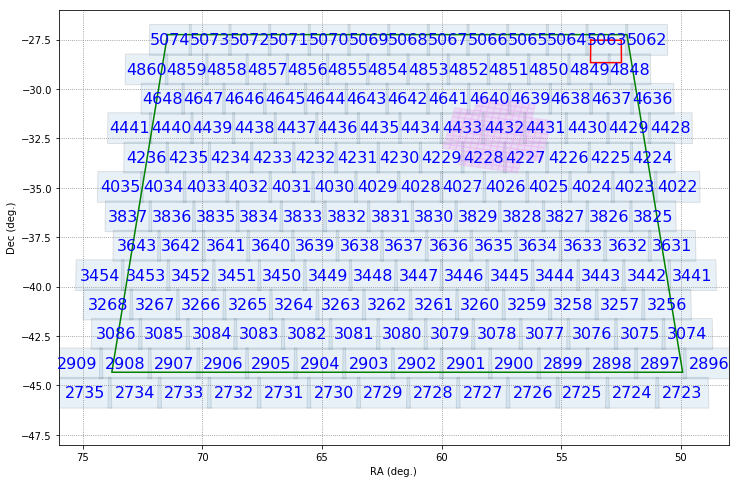
\includegraphics[width=0.8\textwidth]{figs/skymap.png}
    \caption{Sky Map}
    \label{fig:skymap}
\end{figure}



\subsection{Obtaining Data Files via Globus Online}
\label{sec:download}

\subsection{Accessing Data Files via GCRCatalogs}
\label{sec:gcr}



\section{Example Notebooks}
\label{sec:notebooks}

% \section{Validation and Characterization}
% \label{sec:validation}

% \note{MWV: I started this section, but maybe all of this stuff should go in a different paper.  We presented a few things in the DC2 Paper, and we're not going to be exhaustive here.  But I'm in favor of putting something that characterizes the data products in a Note describing the data products.
% We also might want to highlight known things that might otherwise trigger immediate questions.  E.g., the discreteness of the M-type stellar models.}

% \note{YYM: Some of this characterization should go into Sec 2 ``Major Features''}

% \note{MWV: Maybe another more minimally disruptive direction to go would be to include a rendered copy of the Object Table Validation notebook, \code{validate_dc2_run2.2i_object_table.ipynb}, under the Example Notebooks or as an appendix.  Can add the tests Plaszczynski has been doing to this Notebook to help complete things.}

% \note{MWV: 2020-12-15 08:31 EST --  OK.  I didn't get anything extra done last week, so I'll agree that we should remove this "Validation and Characterization" section and go with elements of the Object Table validation notebooks in the examples and mention the discrete M-star models in Section 2.  I've commented out this section.}

% \subsection{Tests of the Object Table}

% These tests can be asked of any coadd catalog from real or simulated data.

% \begin{itemize}
%   \item Do we cover the RA and Dec as expected
%   \item Are stars point-like and galaxies extended?
%   \item Is the distribution of measured PSFs reasonable.  Note that this is on the coadds for the current level of processing, but the coadds should be representative of the distribution of PSFs from the input images.
%   \item Does a color-color diagram of stars look reasonable?
%   \item Are the image 5-sigma point-source depths reasonable?
%   \item Is the areal density of galaxies on the sky reasonable?
%       \begin{itemize}
%           \item Check both versus other surveys using real data of the real sky. 
%       \end{itemize}
%   \item Is the number density of galaxies vs. brightness (say i band magnitude) reasonable?
%       \begin{itemize}
%           \item Check both versus other surveys using real data of the real sky. 
%       \end{itemize}
%   \item Is the separation of stars vs. galaxies decent.  Does it behave as expected as a function of SNR?  Are there unexpected features?
%   \item Is the distribution of shape, ellipticity, and T second moments reasonable and as expected?
%   \item Is the distribution of [shear-based] e1, e2, $e_\text{abs}$ reasonable?  Are there patterns in the distribution across the sky?
%   \item What's the relationship between different types of extended-object photometry?
%   \item Do Central Cluster galaxies follow the red sequence?
%   \begin{itemize}
%       \item Is the cluster red sequence visible in z vs. g-r and r-z vs. g-r plots of extended objects in the data?
%       \item If you run a cluster finder, and then identify central galaxies, do you find that the expected central cluster galaxy red sequence pops out clearly?
%   \end{itemize}

% \end{itemize}

% \subsection{Comparison of the Object Table with Truth}

% Comparison against the known characteristics of the models without matching:

% \begin{itemize}
%   \item Does the areal density of stars match the input model of the Milky Way?
%   \item Does the number density of galaxies vs. brightness (say i band magnitude) match the input model?
% \end{itemize}

% The following questions can only be asked after matching the observered catalog to the truth catalogs.

% \begin{itemize}
%   \item Observed - Truth magnitude
%   \begin{itemize}
%       \item For stars, galaxies.  Point source and extended model photometry.
%       \item Is the distribution centered at 0?
%       \item Is it symmetric or skewed?
%       \item Is the skew consistent with (reverse) Malmquist bias at bright end?
%       \item As a function of brightness.
%         \item Does the scatter at the low SNR end follow the reported uncertainties?
%         \item What happens at the bright end? Are the effects of saturation visible?
%       \item Is a constant offset?  If so, is it consistent with a bookkeeping error somewhere?
%       \item What's the behavior for a SNR > 10 cut.
%   \end{itemize}

%   \item Galaxies
%   \begin{itemize}
%       \item Do Central Cluster galaxies follow the red sequence?
%         \item Look in r-z vs g-r
%         \item This can be done using the truth catalog identify cluster members.  And the presented matched plots
%         \item Compare truth 
%         \item data vs. redshift
%         \item Compare truth -data vs. g-r color.
%         \item This analysis complements the data-only analysis above.
%     \end{itemize}
% \end{itemize}

\section{Conclusion and Outlook}
\label{sec:outlook}


\clearpage

\phantomsection\section*{Acknowledgments}
\addcontentsline{toc}{section}{Acknowledgements}

LSST DESC acknowledges ongoing support from the Institut National de Physique Nucl\'eaire et de Physique des Particules in France; the Science \& Technology Facilities Council in the United Kingdom; and the Department of Energy, the National Science Foundation, and the LSST Corporation in the United States. LSST DESC uses the resources of the IN2P3/CNRS Computing Center (CC-IN2P3--Lyon/Villeurbanne - France) funded by the Centre National de la Recherche Scientifique; the Univ. Savoie Mont Blanc - CNRS/IN2P3 MUST computing center; the National Energy Research Scientific Computing Center, a DOE Office of Science User Facility supported by the Office of Science of the U.S.\ Department of Energy under contract No.\ DE-AC02-05CH11231; STFC DiRAC HPC Facilities, funded by UK BIS National E-infrastructure capital grants; and the UK particle physics grid, supported by the GridPP Collaboration. This research used resources of the Argonne Leadership Computing Facility, which is a DOE Office of Science User Facility supported under Contract DE-AC02-06CH11357. This work was performed in part under DOE contract DE-AC02-76SF00515.


% Individual acknowledgments (sorted by author order)
The work of APH, KH, EK, PL, and ASV at Argonne National Laboratory was supported under the U.S. DOE contract DE-AC02-06CH11357.
Support for YYM was provided by NASA through the NASA Hubble Fellowship grant no.\ HST-HF2-51441.001 awarded by the Space Telescope Science Institute, which is operated by the Association of Universities for Research in Astronomy, Incorporated, under NASA contract NAS5-26555. 



% %%%%%%%% END MATTER
\clearpage


\bibliographystyle{inc/apj-mod}
\phantomsection\bibliography{ref}


\clearpage
\appendix
\renewcommand\thefigure{\thesection\arabic{figure}}
\renewcommand\thetable{\thesection\arabic{table}}
\renewcommand{\thesection}{\Alph{section}}
\renewcommand{\thesubsection}{\Alph{section}\arabic{subsection}}

\phantomsection\section*{Appendices}
\addcontentsline{toc}{section}{Appendices}





\end{document}

% ====================================================================
